\documentclass[12pt, oneside, a4paper]{article}

\usepackage[left=3.5cm, top=2.5cm, bottom=2.5cm, right=2.5cm]{geometry}

\usepackage[utf8]{inputenc}
\usepackage[T1]{polski}
\usepackage[polish]{babel}
\usepackage[]{amsmath}
\usepackage[]{listings}
\usepackage[]{pgf}
\usepackage[]{float}
\usepackage[]{graphics}
\usepackage[]{svg}

\usepackage[
  color=orange!30,
  figcolor=white,
  figwidth=10cm
]{todonotes}

% temporarily for dark background
\usepackage{xcolor}
\definecolor{mybackground}{rgb}{0.15, 0.15, 0.13}
\definecolor{mytext}{rgb}{0.94, 0.94, 0.92}
% \pagecolor{mybackground}
% \color{mytext}

\lstset{
  basicstyle=\ttfamily,
  captionpos=b,
  aboveskip=2em,
}

% listing settings
\renewcommand{\ttdefault}{pcr}
\lstdefinestyle{hls}{
  language=C++,
  keywordstyle=\ttfamily\bfseries,
  numbers=left,
  numberstyle=\small,
  xleftmargin=2em,
}


\begin{document}
\thispagestyle{empty}
\begin{titlepage}
    \begin{center}

      \Large
	    \textbf{Uniwersytet Jagielloński w Krakowie}\vspace{0.2cm}\\ Wydział Fizyki, Astronomii i Informatyki Stosowanej
      \vspace*{1cm}
               
      \vspace{3cm}
      \Large
      \textbf{Wojciech Lepich}\\\vspace{0.5cm}
      \normalsize Nr albumu: 1146600\\
      \vspace{2cm}
      \Huge
      \textbf{Rozpoznawanie cyfr przez sieć neuronową zaimplementowaną na układzie FPGA}
      
      \vspace{1.5cm}
      \normalsize
      Praca licencjacka\\
      na kierunku Informatyka\\ \vspace{0.15cm}
        
      \vfill
      \vspace{2cm}
      \begin{minipage}{1\textwidth}
\begin{flushright}
Praca wykonana pod kierunkiem\\
dr. Grzegorza Korcyla\\
z Zakładu Technologii Informatycznych
\end{flushright}
\end{minipage}
        
        \vspace{2cm}
        \begin{center}
      Kraków 2020
        \end{center}
    \end{center}
\end{titlepage}

\newpage 
\thispagestyle{empty}
\vspace{2.5cm}
\begin{flushleft}
\large \textbf{Oświadczenie autora pracy}\vspace{0.6cm}\\
\end{flushleft}

\noindent Świadom odpowiedzialności prawnej oświadczam, że niniejsza praca dyplomowa została napisana przeze mnie samodzielnie i nie zawiera treści uzyskanych w sposób niezgodny z obowiązującymi przepisami.\\

\noindent Oświadczam również, że przedstawiona praca nie była wcześniej przedmiotem procedur związanych z uzyskaniem tytułu zawodowego w wyższej uczelni.
\vspace{2cm}
\begin{center}
\begin{tabular}{lr}
\ldots\ldots\ldots\ldots\ldots\ldots~~~~~~~~~~~~~~~~~~~~~~~~~~~~~~~~~~~~~~&
\ldots\ldots\ldots\ldots\ldots\ldots\ldots\ldots\ldots \\
{~~~~Kraków, dnia} & {Podpis autora pracy~~~~}
\end{tabular}
\end{center}
\vspace{5cm}
\begin{flushleft}
\large \textbf{Oświadczenie kierującego pracą}
\end{flushleft}

\noindent Potwierdzam, że niniejsza praca została przygotowana pod moim kierunkiem i~kwalifikuje się do przedstawienia jej w postępowaniu o nadanie tytułu zawodowego.
\vspace{2cm}
\begin{center}
\begin{tabular}{lr}
\ldots\ldots\ldots\ldots\ldots\ldots~~~~~~~~~~~~~~~~~~~~~~~~~~~~~~~~~~~~~~&
\ldots\ldots\ldots\ldots\ldots\ldots\ldots\ldots\ldots \\
{~~~~Kraków, dnia} & {Podpis kierującego pracą~~}
\end{tabular}
\end{center}
\vfill

\newpage
\tableofcontents

\newpage
\section{Wstęp}
Tutaj wstęp

\newpage
\section{Teoria}
\subsection{Architektura FPGA}
Field-Programmable Gate Array (FPGA) to układy scalone, które mogą być
elektronicznie przeprogramowane bez potrzeby demontażu samego układu
z urządzenia. W porównaniu do układów ASIC znacznie taniej zaprojektować
pierwszy działający układ. Elastyczna natura układów FPGA wiąże się z większym
zużyciem powierzchni krzemu, opóźnień oraz zużycia energii.
\todo{Dodać przypis} (FPGA architecture: survey and challenges)

Podstawowa struktura układów FPGA składa się z różnych bloków logicznych,
które mogą być łączone ze sobą w zależności od wymagań projektowych.
Przykładami takich bloków są:
DSP (jednostka przeprowadzająca obliczenia dodawania/mnożenia),
LUT (Look-Up Table, de facto tablica prawdy dowolnej funkcji boolowskiej),
Flip Flop (przechowują wynik LUT), BRAM (Block RAM, pamięć dwuportowa,
jest w stanie przechowywać względnie dużą ilość danych).

Układy FPGA przeważnie pracują na kilku-, kilkunastukrotnie niższych
częstotliwościach niż CPU. Osiągają wysoką wydajność
dzięki masywnemu zrównolegleniu obliczeń.

\subsection{Przetwarzanie obrazu}
Cyfrowe przetwarzanie obrazu jest problemem wymagającym dużych mocy
obliczeniowych ze względu na ilość danych do przetworzenia. Nieskompresowany
kolorowy obraz z pikselami w formacie RGB (po 8 bitów na kolor) o wysokości
720 pikseli i szerokości 1280 pikseli to 22118400 bitów (\(\approx \) 2,5MB). Obraz
przetwarzany w czasie rzeczywistym, na przykład z kamery, zwielokrotnia tę
liczbę o liczbę klatek na sekundę (przy trzydziestu klatkach na sekundę liczba
danych rośnie do około 79 megabajtów na sekundę). Należy również pamiętać, że
dane są dwuwymiarowe co jest ważne przy problemach związanych z rozpoznawaniem
wzorców, klasyfikacją przedmiotów na obrazie, filtrowania w celu rozmazania lub
wyostrzenia obrazów, itp.

\subsubsection{Formaty pikseli}
Jest wiele modeli przestrzeni barw (a co za tym idzie, sposobów kodowania
pikseli) między innymi:
\begin{itemize}
  \item RGB, używany w aparatach, skanerach, telewizorach
  \item CMYK, używany w druku wielobarwnym
  \item HSV
  \item YUV
\end{itemize}
Składowe dwóch ostatnich przestrzeni barw oddzielają informację o jasności
od informacji o kolorach. Model barw YUV składa się z kanału luminacji Y
oraz kanałów kodujących barwę U oraz V, są to kolejno składowa niebieska
i składowa czerwona. W projekcie użyty jest format pikseli YUY2 (znany też
pod nazwą YUYV), w którym na dwa piksele przypadają 32 bity.
\begin{figure}[h]
  \centering
  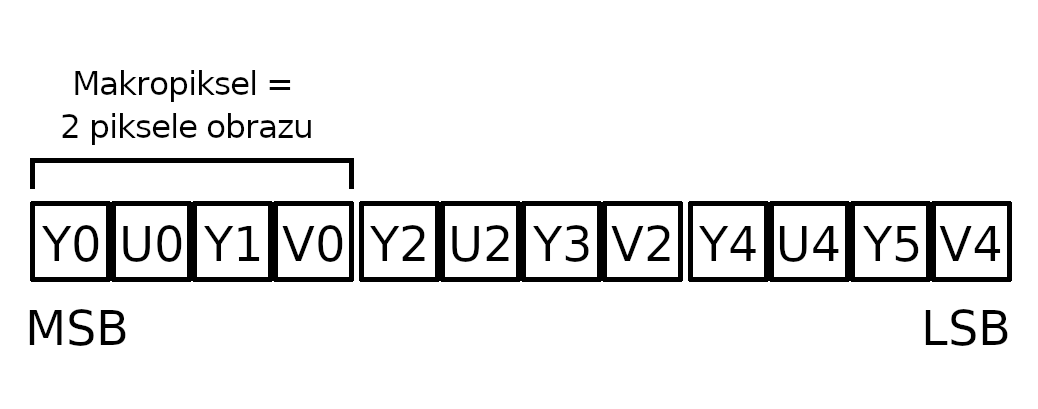
\includegraphics[scale=1.2]{figures/yuv2-scheme.png} 
  \caption{Schemat formatu pikseli YUV2}\label{fig:yuv2}
\end{figure}
Licząc od najstarszego bitu pierwsze osiem bitów przypada na Y0, to jest
luminacja pierwszego piksela, następne osiem bitów na U0, kolejne osiem bitów
to luminacja drugiego piksela, a pozostałe bity to składowa czerwona V0.
Dla obydwóch pikseli składowe U i V są wspólne. Co istotne w projekcie,
łatwo oddzielić luminację, która jest używana w przetwarzaniu obrazu.

\subsection{Sieci neuronowe}
Sztuczna sieć neuronowa (SSN) jest modelem zdolnym do odwzorowania złożonych
funkcji. Najprostsze sieci są zbudowane ze sztucznych neuronów, z których każdy
posiada wiele wejść oraz jedno wyjście, które może być połączone z wejściami
wielu innych neuronów. Każde z wejść neuronu jest związane ze znalezioną
w procesie trenowania wagą. Wartość wyjścia to obliczony wynik funkcji aktywacji
z sumy ważonych wejść. Sieć może mieć wiele warstw neuronów ukrytych, których
wejściami są wyjścia neuronów z poprzedniej warstwy. 

Sieci neuronowe są stosowane w problemach
związanych z predykcją, klasyfikacją, przetwarzaniem i analizowaniem
danych. Do ich zastosowania nie jest potrzebna znajomość algorytmu rozwiązania
danego problemu. Obliczenia w sieciach są wykonywane równolegle w każdej
warstwie, dzięki czemu implementacja sieci na układzie FPGA może działać
wielokrotnie szybciej niż na CPU, pomimo niższej częstotliwości układu.

\newpage
\section{Opis projektu}

\subsection{Zarys projektu}
Celem projektu jest implementacja systemu do rozpoznawania cyfr
w czasie rzeczywistym. Cel zrealizowano poprzez implementację
wtyczki GStreamera, wykorzystującej sieć neuronową, na układzie
Xilinx Zynq MPSoC oraz stworzenie odpowiedniego potoku danych
korzystając z bibliotek GStreamer. Zadaniami spoczywającymi na innych
elementach potoku jest obsługa kamery,
kadrowanie i skalowanie obrazu oraz wyświetlenie go na końcowym urządzeniu.

\subsection{Platforma}
\missingfigure{Zdjęcie stanowiska}
Sprzęt wykorzystany w projekcie to Xilinx Zynq UltraScale+ MPSoC ZCU104.
Na jednym układzie znajduje się czterordzeniowy procesor
ARM \mbox{Cortex-A53},
dwurdzeniowy procesor ARM \mbox{Cortex-R5},
układ graficzny \mbox{Mali-400} oraz zasoby FPGA.
Całość projektu została oparta o platformę Xilinx reVISION. Przetwarzane
dane dostarczane są z kamery USB, która była dołączona w zestawie z płytą Zynq.
Urządzeniem końcowym jest telewizor połączony przewodem HDMI z płytą.

\subsection{Sieć neuronowa}
Architektura sieci została dobrana uwzględniając dostępne zasoby programowalnej
logiki na płycie, a także możliwości sprzętu na którym dokonywana była jej
synteza. Dla problemu klasyfikowania obrazów dobrze nadają się sieci
splotowe (konwolucyjne, ang.\ convolutional neural networks --- CNN), 
\todo{przypis} których przykładem jest popularna sieć \mbox{LeNet-5}.
Architektura ta zawiera zarówno w pełni połączone warstwy
oraz warstwy splotowe i łączące.
Niestety z powodu ograniczeń sprzętowych w pracy nie została użyta ta
architektura.

\begin{figure}[h]
  \centering
  \includesvg[scale=0.5625]{figures/nn-scheme.svg}
  \caption{Schemat użytej architektury.
  }\label{fig:nn-scheme}
\end{figure}
Model wykorzystany w projekcie posiada 2 warstwy ukryte, posiadające kolejno
12 i 40 neuronów aktywowanych funkcją ReLU, i warstwy wyjściowej złożonej
z 10 neuronów z funkcją aktywacji softmax. Do stworzenia sieci wykorzystano
bibliotekę TensorFlow. Sieć uczona była na danych
z \todo{przypis}bazy MNIST składającej się łącznie z 70000 przykładów
cyfr na obrazach o wielkości 28\(\times \)28 pikseli, z których każdy
przedstawiony jest jako wartość od 0 (kolor czarny) do 255 (kolor biały).
Próbki zostały
podzielone na zbiór uczący, liczący 60000 próbek, oraz zbiór do testów
z pozostałych 10000 cyfr.

Oryginalnie cyfry są białe na czarnym tle co zwiększa
\todo{przypis - badania własne} dokładność działania sieci (więcej 0 w danych),
natomiast trzeba wziąć to pod uwagę przy późniejszym wykorzystaniu sieci,
ponieważ docelowo sieć ma rozpoznawać czarne cyfry na białym tle.

\subsection{hls4ml}
\subsubsection{Idea hls4ml}
\todo[inline]{Czy mogę użyć tego schematu? Lub pod jakimi warunkami mogę?
Obrazek jest z dokumentacji hls4ml}
\begin{figure}[h]
  \centering
  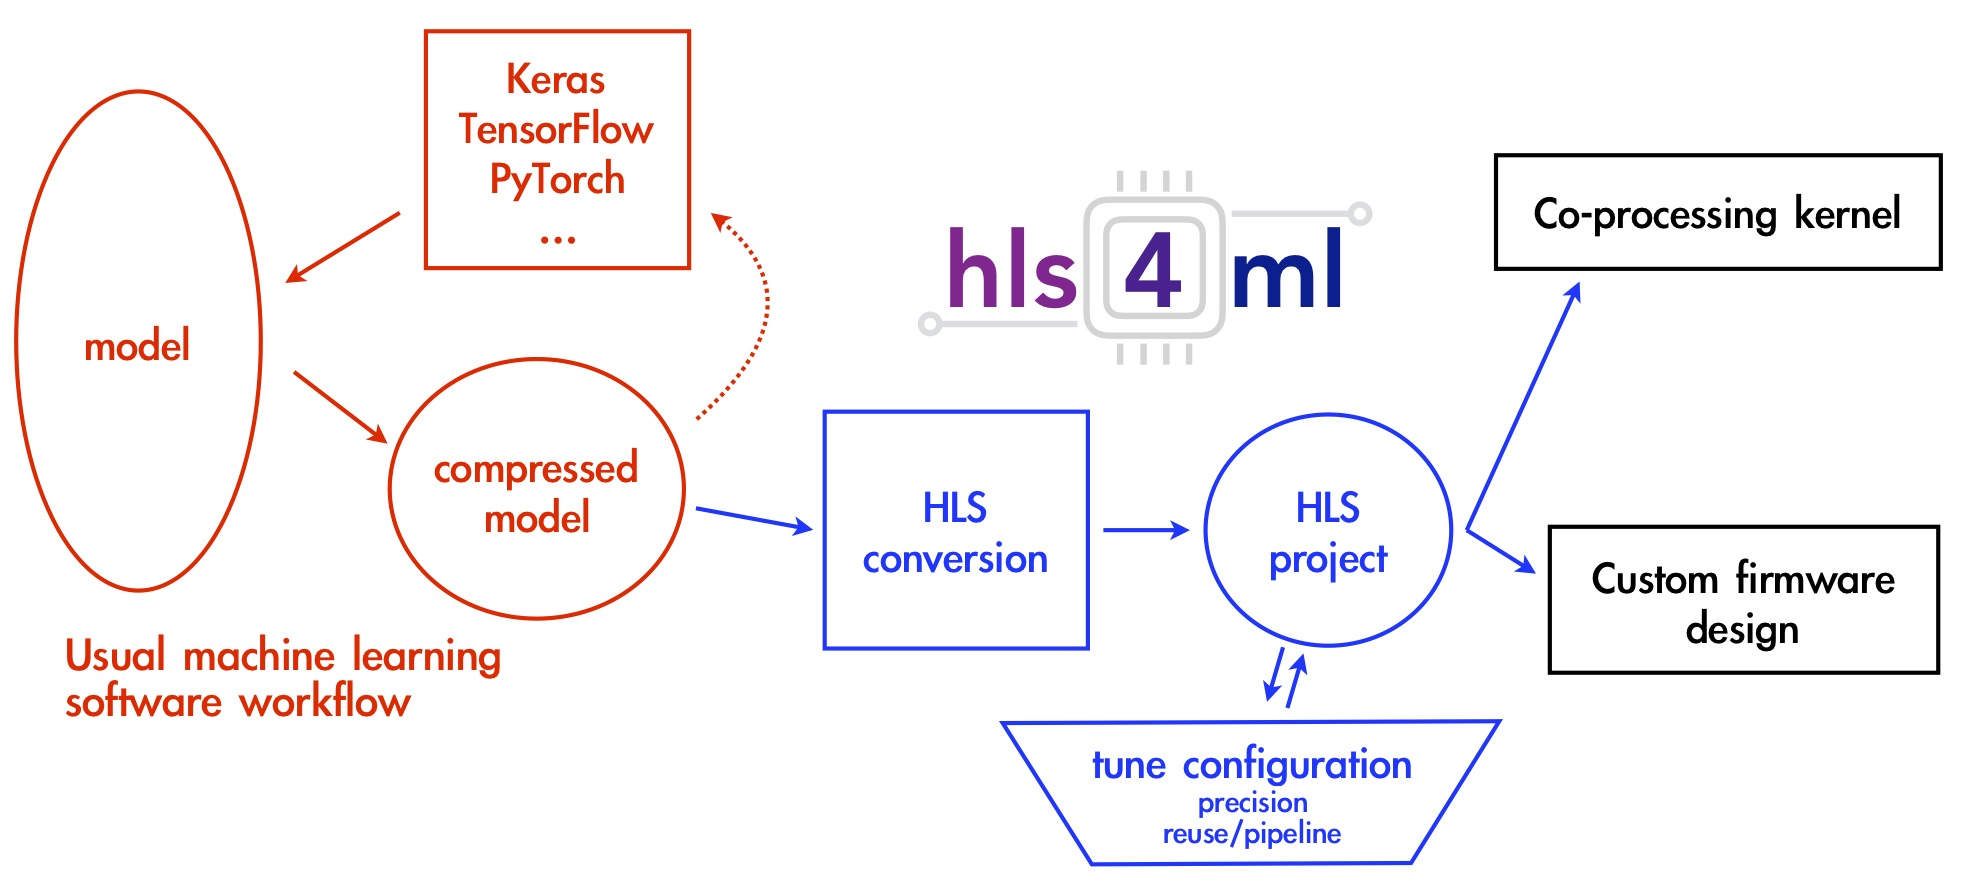
\includegraphics[scale=0.2]{figures/hls4ml.jpg}
  \caption{Schemat pracy z hls4ml}\label{fig:hls4ml}
\end{figure}
Celem projektu hls4ml jest automatyczne przetłumaczenie wytrenowanego modelu,
architektury i wag, do projektu syntezy wysokiego poziomu (HLS).
Czerwona część schematu pokazuje ogólną organizację pracy przy projektowaniu 
odpowiedniego modelu uczenia maszynowego. Niebieska część należy do hls4ml,
który tłumaczy dostarczony model z wagami do syntetyzowalnego kodu, który
następnie można włączyć do większego projektu lub zaimplementować jako
samodzielną część na FPGA. Generowany projekt jest parametryzowany
przez plik konfiguracyjny yml zawierający ścieżkę do pliku z zapisanym modelem
wraz z wagami, typy danych kodujące wartości wag, nazwę docelowego układu FPGA.

\subsubsection{Precyzja danych}
Typ danych używany w przekonwertowanym modelu to duże liczby całkowite
(\lstinline{ap_int}) oraz liczby stałoprzecinkowe (\lstinline{ap_fixed}).
Precyzję obu można ustalić do jednego bita.
\todo{Poprawić wystający tekst}
Obliczenia przeprowadzane na liczbach o mniejszej
precyzji są szybsze, natomiast zbyt niska może poskutkować
bezużytecznością zsyntetyzowanej sieci. Aby odpowiednio dobrać precyzję
wag skorzystano z pythonowej biblioteki hls4ml.profiling.

Program korzystający z funkcji dostarczanych przez tę bibliotekę
analizuje plik konfiguracyjny yml oraz model z pliku h5.
Wynikiem działania programu jest wykres przedstawiający
rozkład wartości wag każdej z warstw modelu otrzymanych w procesie trenowania.
Szare pole w tle wykresu
przedstawia zakres wartości, które obejmowane są przez precyzję określoną
w pliku konfiguracyjnym. Dobrym punktem początkowym jest wybranie takiej
liczby bitów dla każdej z warstw, która obejmuje wszystkie możliwe wagi.
Dalsze ustalanie precyzji można wykonać w trakcie analizy wyników
symulacji.
\begin{figure}[H]
  \caption{Rozkład wartości wag modelu}\label{fig:weights_dist}
  %% Creator: Matplotlib, PGF backend
%%
%% To include the figure in your LaTeX document, write
%%   \input{<filename>.pgf}
%%
%% Make sure the required packages are loaded in your preamble
%%   \usepackage{pgf}
%%
%% Figures using additional raster images can only be included by \input if
%% they are in the same directory as the main LaTeX file. For loading figures
%% from other directories you can use the `import` package
%%   \usepackage{import}
%% and then include the figures with
%%   \import{<path to file>}{<filename>.pgf}
%%
%% Matplotlib used the following preamble
%%   \usepackage{fontspec}
%%   \setmainfont{DejaVuSerif.ttf}[Path=/home/wojtek/miniconda3/envs/hls4ml_prof/lib/python3.6/site-packages/matplotlib/mpl-data/fonts/ttf/]
%%   \setsansfont{DejaVuSans.ttf}[Path=/home/wojtek/miniconda3/envs/hls4ml_prof/lib/python3.6/site-packages/matplotlib/mpl-data/fonts/ttf/]
%%   \setmonofont{DejaVuSansMono.ttf}[Path=/home/wojtek/miniconda3/envs/hls4ml_prof/lib/python3.6/site-packages/matplotlib/mpl-data/fonts/ttf/]
%%
\begingroup%
\makeatletter%
\begin{pgfpicture}%
\pgfpathrectangle{\pgfpointorigin}{\pgfqpoint{5.400000in}{4.000000in}}%
\pgfusepath{use as bounding box, clip}%
\begin{pgfscope}%
\pgfsetbuttcap%
\pgfsetmiterjoin%
\definecolor{currentfill}{rgb}{1.000000,1.000000,1.000000}%
\pgfsetfillcolor{currentfill}%
\pgfsetlinewidth{0.000000pt}%
\definecolor{currentstroke}{rgb}{1.000000,1.000000,1.000000}%
\pgfsetstrokecolor{currentstroke}%
\pgfsetdash{}{0pt}%
\pgfpathmoveto{\pgfqpoint{0.000000in}{0.000000in}}%
\pgfpathlineto{\pgfqpoint{5.400000in}{0.000000in}}%
\pgfpathlineto{\pgfqpoint{5.400000in}{4.000000in}}%
\pgfpathlineto{\pgfqpoint{0.000000in}{4.000000in}}%
\pgfpathclose%
\pgfusepath{fill}%
\end{pgfscope}%
\begin{pgfscope}%
\pgfsetbuttcap%
\pgfsetmiterjoin%
\definecolor{currentfill}{rgb}{1.000000,1.000000,1.000000}%
\pgfsetfillcolor{currentfill}%
\pgfsetlinewidth{0.000000pt}%
\definecolor{currentstroke}{rgb}{0.000000,0.000000,0.000000}%
\pgfsetstrokecolor{currentstroke}%
\pgfsetstrokeopacity{0.000000}%
\pgfsetdash{}{0pt}%
\pgfpathmoveto{\pgfqpoint{0.808711in}{0.523981in}}%
\pgfpathlineto{\pgfqpoint{5.273438in}{0.523981in}}%
\pgfpathlineto{\pgfqpoint{5.273438in}{3.705556in}}%
\pgfpathlineto{\pgfqpoint{0.808711in}{3.705556in}}%
\pgfpathclose%
\pgfusepath{fill}%
\end{pgfscope}%
\begin{pgfscope}%
\pgfpathrectangle{\pgfqpoint{0.808711in}{0.523981in}}{\pgfqpoint{4.464727in}{3.181574in}}%
\pgfusepath{clip}%
\pgfsetbuttcap%
\pgfsetmiterjoin%
\definecolor{currentfill}{rgb}{0.840692,0.901638,0.958662}%
\pgfsetfillcolor{currentfill}%
\pgfsetlinewidth{1.003750pt}%
\definecolor{currentstroke}{rgb}{0.840692,0.901638,0.958662}%
\pgfsetstrokecolor{currentstroke}%
\pgfsetdash{}{0pt}%
\pgfpathmoveto{\pgfqpoint{3.668229in}{0.683060in}}%
\pgfpathlineto{\pgfqpoint{3.777437in}{0.683060in}}%
\pgfpathlineto{\pgfqpoint{3.777437in}{1.001218in}}%
\pgfpathlineto{\pgfqpoint{3.668229in}{1.001218in}}%
\pgfpathclose%
\pgfusepath{stroke,fill}%
\end{pgfscope}%
\begin{pgfscope}%
\pgfpathrectangle{\pgfqpoint{0.808711in}{0.523981in}}{\pgfqpoint{4.464727in}{3.181574in}}%
\pgfusepath{clip}%
\pgfsetbuttcap%
\pgfsetmiterjoin%
\definecolor{currentfill}{rgb}{0.671895,0.814379,0.900654}%
\pgfsetfillcolor{currentfill}%
\pgfsetlinewidth{1.003750pt}%
\definecolor{currentstroke}{rgb}{0.671895,0.814379,0.900654}%
\pgfsetstrokecolor{currentstroke}%
\pgfsetdash{}{0pt}%
\pgfpathmoveto{\pgfqpoint{3.484240in}{1.319375in}}%
\pgfpathlineto{\pgfqpoint{3.717507in}{1.319375in}}%
\pgfpathlineto{\pgfqpoint{3.717507in}{1.637532in}}%
\pgfpathlineto{\pgfqpoint{3.484240in}{1.637532in}}%
\pgfpathclose%
\pgfusepath{stroke,fill}%
\end{pgfscope}%
\begin{pgfscope}%
\pgfpathrectangle{\pgfqpoint{0.808711in}{0.523981in}}{\pgfqpoint{4.464727in}{3.181574in}}%
\pgfusepath{clip}%
\pgfsetbuttcap%
\pgfsetmiterjoin%
\definecolor{currentfill}{rgb}{0.417086,0.680631,0.838231}%
\pgfsetfillcolor{currentfill}%
\pgfsetlinewidth{1.003750pt}%
\definecolor{currentstroke}{rgb}{0.417086,0.680631,0.838231}%
\pgfsetstrokecolor{currentstroke}%
\pgfsetdash{}{0pt}%
\pgfpathmoveto{\pgfqpoint{3.184987in}{1.955690in}}%
\pgfpathlineto{\pgfqpoint{3.785356in}{1.955690in}}%
\pgfpathlineto{\pgfqpoint{3.785356in}{2.273847in}}%
\pgfpathlineto{\pgfqpoint{3.184987in}{2.273847in}}%
\pgfpathclose%
\pgfusepath{stroke,fill}%
\end{pgfscope}%
\begin{pgfscope}%
\pgfpathrectangle{\pgfqpoint{0.808711in}{0.523981in}}{\pgfqpoint{4.464727in}{3.181574in}}%
\pgfusepath{clip}%
\pgfsetbuttcap%
\pgfsetmiterjoin%
\definecolor{currentfill}{rgb}{0.215686,0.529412,0.754248}%
\pgfsetfillcolor{currentfill}%
\pgfsetlinewidth{1.003750pt}%
\definecolor{currentstroke}{rgb}{0.215686,0.529412,0.754248}%
\pgfsetstrokecolor{currentstroke}%
\pgfsetdash{}{0pt}%
\pgfpathmoveto{\pgfqpoint{3.444094in}{2.592005in}}%
\pgfpathlineto{\pgfqpoint{3.788213in}{2.592005in}}%
\pgfpathlineto{\pgfqpoint{3.788213in}{2.910162in}}%
\pgfpathlineto{\pgfqpoint{3.444094in}{2.910162in}}%
\pgfpathclose%
\pgfusepath{stroke,fill}%
\end{pgfscope}%
\begin{pgfscope}%
\pgfpathrectangle{\pgfqpoint{0.808711in}{0.523981in}}{\pgfqpoint{4.464727in}{3.181574in}}%
\pgfusepath{clip}%
\pgfsetbuttcap%
\pgfsetmiterjoin%
\definecolor{currentfill}{rgb}{0.062514,0.357509,0.642907}%
\pgfsetfillcolor{currentfill}%
\pgfsetlinewidth{1.003750pt}%
\definecolor{currentstroke}{rgb}{0.062514,0.357509,0.642907}%
\pgfsetstrokecolor{currentstroke}%
\pgfsetdash{}{0pt}%
\pgfpathmoveto{\pgfqpoint{3.360485in}{3.228319in}}%
\pgfpathlineto{\pgfqpoint{3.656129in}{3.228319in}}%
\pgfpathlineto{\pgfqpoint{3.656129in}{3.546477in}}%
\pgfpathlineto{\pgfqpoint{3.360485in}{3.546477in}}%
\pgfpathclose%
\pgfusepath{stroke,fill}%
\end{pgfscope}%
\begin{pgfscope}%
\pgfpathrectangle{\pgfqpoint{0.808711in}{0.523981in}}{\pgfqpoint{4.464727in}{3.181574in}}%
\pgfusepath{clip}%
\pgfsetbuttcap%
\pgfsetmiterjoin%
\definecolor{currentfill}{rgb}{0.501961,0.501961,0.501961}%
\pgfsetfillcolor{currentfill}%
\pgfsetfillopacity{0.200000}%
\pgfsetlinewidth{1.003750pt}%
\definecolor{currentstroke}{rgb}{0.501961,0.501961,0.501961}%
\pgfsetstrokecolor{currentstroke}%
\pgfsetstrokeopacity{0.200000}%
\pgfsetdash{}{0pt}%
\pgfpathmoveto{\pgfqpoint{0.917817in}{3.132872in}}%
\pgfpathlineto{\pgfqpoint{4.323132in}{3.132872in}}%
\pgfpathlineto{\pgfqpoint{4.323132in}{3.641924in}}%
\pgfpathlineto{\pgfqpoint{0.917817in}{3.641924in}}%
\pgfpathclose%
\pgfusepath{stroke,fill}%
\end{pgfscope}%
\begin{pgfscope}%
\pgfpathrectangle{\pgfqpoint{0.808711in}{0.523981in}}{\pgfqpoint{4.464727in}{3.181574in}}%
\pgfusepath{clip}%
\pgfsetbuttcap%
\pgfsetmiterjoin%
\definecolor{currentfill}{rgb}{0.501961,0.501961,0.501961}%
\pgfsetfillcolor{currentfill}%
\pgfsetfillopacity{0.200000}%
\pgfsetlinewidth{1.003750pt}%
\definecolor{currentstroke}{rgb}{0.501961,0.501961,0.501961}%
\pgfsetstrokecolor{currentstroke}%
\pgfsetstrokeopacity{0.200000}%
\pgfsetdash{}{0pt}%
\pgfpathmoveto{\pgfqpoint{0.917817in}{2.496557in}}%
\pgfpathlineto{\pgfqpoint{4.323132in}{2.496557in}}%
\pgfpathlineto{\pgfqpoint{4.323132in}{3.005609in}}%
\pgfpathlineto{\pgfqpoint{0.917817in}{3.005609in}}%
\pgfpathclose%
\pgfusepath{stroke,fill}%
\end{pgfscope}%
\begin{pgfscope}%
\pgfpathrectangle{\pgfqpoint{0.808711in}{0.523981in}}{\pgfqpoint{4.464727in}{3.181574in}}%
\pgfusepath{clip}%
\pgfsetbuttcap%
\pgfsetmiterjoin%
\definecolor{currentfill}{rgb}{0.501961,0.501961,0.501961}%
\pgfsetfillcolor{currentfill}%
\pgfsetfillopacity{0.200000}%
\pgfsetlinewidth{1.003750pt}%
\definecolor{currentstroke}{rgb}{0.501961,0.501961,0.501961}%
\pgfsetstrokecolor{currentstroke}%
\pgfsetstrokeopacity{0.200000}%
\pgfsetdash{}{0pt}%
\pgfpathmoveto{\pgfqpoint{2.172406in}{1.860243in}}%
\pgfpathlineto{\pgfqpoint{5.219267in}{1.860243in}}%
\pgfpathlineto{\pgfqpoint{5.219267in}{2.369294in}}%
\pgfpathlineto{\pgfqpoint{2.172406in}{2.369294in}}%
\pgfpathclose%
\pgfusepath{stroke,fill}%
\end{pgfscope}%
\begin{pgfscope}%
\pgfpathrectangle{\pgfqpoint{0.808711in}{0.523981in}}{\pgfqpoint{4.464727in}{3.181574in}}%
\pgfusepath{clip}%
\pgfsetbuttcap%
\pgfsetmiterjoin%
\definecolor{currentfill}{rgb}{0.501961,0.501961,0.501961}%
\pgfsetfillcolor{currentfill}%
\pgfsetfillopacity{0.200000}%
\pgfsetlinewidth{1.003750pt}%
\definecolor{currentstroke}{rgb}{0.501961,0.501961,0.501961}%
\pgfsetstrokecolor{currentstroke}%
\pgfsetstrokeopacity{0.200000}%
\pgfsetdash{}{0pt}%
\pgfpathmoveto{\pgfqpoint{1.993179in}{1.223928in}}%
\pgfpathlineto{\pgfqpoint{4.323132in}{1.223928in}}%
\pgfpathlineto{\pgfqpoint{4.323132in}{1.732980in}}%
\pgfpathlineto{\pgfqpoint{1.993179in}{1.732980in}}%
\pgfpathclose%
\pgfusepath{stroke,fill}%
\end{pgfscope}%
\begin{pgfscope}%
\pgfpathrectangle{\pgfqpoint{0.808711in}{0.523981in}}{\pgfqpoint{4.464727in}{3.181574in}}%
\pgfusepath{clip}%
\pgfsetbuttcap%
\pgfsetmiterjoin%
\definecolor{currentfill}{rgb}{0.501961,0.501961,0.501961}%
\pgfsetfillcolor{currentfill}%
\pgfsetfillopacity{0.200000}%
\pgfsetlinewidth{1.003750pt}%
\definecolor{currentstroke}{rgb}{0.501961,0.501961,0.501961}%
\pgfsetstrokecolor{currentstroke}%
\pgfsetstrokeopacity{0.200000}%
\pgfsetdash{}{0pt}%
\pgfpathmoveto{\pgfqpoint{3.426996in}{0.587613in}}%
\pgfpathlineto{\pgfqpoint{4.323132in}{0.587613in}}%
\pgfpathlineto{\pgfqpoint{4.323132in}{1.096665in}}%
\pgfpathlineto{\pgfqpoint{3.426996in}{1.096665in}}%
\pgfpathclose%
\pgfusepath{stroke,fill}%
\end{pgfscope}%
\begin{pgfscope}%
\pgfsetbuttcap%
\pgfsetroundjoin%
\definecolor{currentfill}{rgb}{0.000000,0.000000,0.000000}%
\pgfsetfillcolor{currentfill}%
\pgfsetlinewidth{0.803000pt}%
\definecolor{currentstroke}{rgb}{0.000000,0.000000,0.000000}%
\pgfsetstrokecolor{currentstroke}%
\pgfsetdash{}{0pt}%
\pgfsys@defobject{currentmarker}{\pgfqpoint{0.000000in}{-0.048611in}}{\pgfqpoint{0.000000in}{0.000000in}}{%
\pgfpathmoveto{\pgfqpoint{0.000000in}{0.000000in}}%
\pgfpathlineto{\pgfqpoint{0.000000in}{-0.048611in}}%
\pgfusepath{stroke,fill}%
}%
\begin{pgfscope}%
\pgfsys@transformshift{1.276271in}{0.523981in}%
\pgfsys@useobject{currentmarker}{}%
\end{pgfscope}%
\end{pgfscope}%
\begin{pgfscope}%
\definecolor{textcolor}{rgb}{0.000000,0.000000,0.000000}%
\pgfsetstrokecolor{textcolor}%
\pgfsetfillcolor{textcolor}%
\pgftext[x=1.276271in,y=0.426759in,,top]{\color{textcolor}\sffamily\fontsize{10.000000}{12.000000}\selectfont \(\displaystyle {2^{-18}}\)}%
\end{pgfscope}%
\begin{pgfscope}%
\pgfsetbuttcap%
\pgfsetroundjoin%
\definecolor{currentfill}{rgb}{0.000000,0.000000,0.000000}%
\pgfsetfillcolor{currentfill}%
\pgfsetlinewidth{0.803000pt}%
\definecolor{currentstroke}{rgb}{0.000000,0.000000,0.000000}%
\pgfsetstrokecolor{currentstroke}%
\pgfsetdash{}{0pt}%
\pgfsys@defobject{currentmarker}{\pgfqpoint{0.000000in}{-0.048611in}}{\pgfqpoint{0.000000in}{0.000000in}}{%
\pgfpathmoveto{\pgfqpoint{0.000000in}{0.000000in}}%
\pgfpathlineto{\pgfqpoint{0.000000in}{-0.048611in}}%
\pgfusepath{stroke,fill}%
}%
\begin{pgfscope}%
\pgfsys@transformshift{1.813952in}{0.523981in}%
\pgfsys@useobject{currentmarker}{}%
\end{pgfscope}%
\end{pgfscope}%
\begin{pgfscope}%
\definecolor{textcolor}{rgb}{0.000000,0.000000,0.000000}%
\pgfsetstrokecolor{textcolor}%
\pgfsetfillcolor{textcolor}%
\pgftext[x=1.813952in,y=0.426759in,,top]{\color{textcolor}\sffamily\fontsize{10.000000}{12.000000}\selectfont \(\displaystyle {2^{-15}}\)}%
\end{pgfscope}%
\begin{pgfscope}%
\pgfsetbuttcap%
\pgfsetroundjoin%
\definecolor{currentfill}{rgb}{0.000000,0.000000,0.000000}%
\pgfsetfillcolor{currentfill}%
\pgfsetlinewidth{0.803000pt}%
\definecolor{currentstroke}{rgb}{0.000000,0.000000,0.000000}%
\pgfsetstrokecolor{currentstroke}%
\pgfsetdash{}{0pt}%
\pgfsys@defobject{currentmarker}{\pgfqpoint{0.000000in}{-0.048611in}}{\pgfqpoint{0.000000in}{0.000000in}}{%
\pgfpathmoveto{\pgfqpoint{0.000000in}{0.000000in}}%
\pgfpathlineto{\pgfqpoint{0.000000in}{-0.048611in}}%
\pgfusepath{stroke,fill}%
}%
\begin{pgfscope}%
\pgfsys@transformshift{2.351633in}{0.523981in}%
\pgfsys@useobject{currentmarker}{}%
\end{pgfscope}%
\end{pgfscope}%
\begin{pgfscope}%
\definecolor{textcolor}{rgb}{0.000000,0.000000,0.000000}%
\pgfsetstrokecolor{textcolor}%
\pgfsetfillcolor{textcolor}%
\pgftext[x=2.351633in,y=0.426759in,,top]{\color{textcolor}\sffamily\fontsize{10.000000}{12.000000}\selectfont \(\displaystyle {2^{-12}}\)}%
\end{pgfscope}%
\begin{pgfscope}%
\pgfsetbuttcap%
\pgfsetroundjoin%
\definecolor{currentfill}{rgb}{0.000000,0.000000,0.000000}%
\pgfsetfillcolor{currentfill}%
\pgfsetlinewidth{0.803000pt}%
\definecolor{currentstroke}{rgb}{0.000000,0.000000,0.000000}%
\pgfsetstrokecolor{currentstroke}%
\pgfsetdash{}{0pt}%
\pgfsys@defobject{currentmarker}{\pgfqpoint{0.000000in}{-0.048611in}}{\pgfqpoint{0.000000in}{0.000000in}}{%
\pgfpathmoveto{\pgfqpoint{0.000000in}{0.000000in}}%
\pgfpathlineto{\pgfqpoint{0.000000in}{-0.048611in}}%
\pgfusepath{stroke,fill}%
}%
\begin{pgfscope}%
\pgfsys@transformshift{2.889315in}{0.523981in}%
\pgfsys@useobject{currentmarker}{}%
\end{pgfscope}%
\end{pgfscope}%
\begin{pgfscope}%
\definecolor{textcolor}{rgb}{0.000000,0.000000,0.000000}%
\pgfsetstrokecolor{textcolor}%
\pgfsetfillcolor{textcolor}%
\pgftext[x=2.889315in,y=0.426759in,,top]{\color{textcolor}\sffamily\fontsize{10.000000}{12.000000}\selectfont \(\displaystyle {2^{-9}}\)}%
\end{pgfscope}%
\begin{pgfscope}%
\pgfsetbuttcap%
\pgfsetroundjoin%
\definecolor{currentfill}{rgb}{0.000000,0.000000,0.000000}%
\pgfsetfillcolor{currentfill}%
\pgfsetlinewidth{0.803000pt}%
\definecolor{currentstroke}{rgb}{0.000000,0.000000,0.000000}%
\pgfsetstrokecolor{currentstroke}%
\pgfsetdash{}{0pt}%
\pgfsys@defobject{currentmarker}{\pgfqpoint{0.000000in}{-0.048611in}}{\pgfqpoint{0.000000in}{0.000000in}}{%
\pgfpathmoveto{\pgfqpoint{0.000000in}{0.000000in}}%
\pgfpathlineto{\pgfqpoint{0.000000in}{-0.048611in}}%
\pgfusepath{stroke,fill}%
}%
\begin{pgfscope}%
\pgfsys@transformshift{3.426996in}{0.523981in}%
\pgfsys@useobject{currentmarker}{}%
\end{pgfscope}%
\end{pgfscope}%
\begin{pgfscope}%
\definecolor{textcolor}{rgb}{0.000000,0.000000,0.000000}%
\pgfsetstrokecolor{textcolor}%
\pgfsetfillcolor{textcolor}%
\pgftext[x=3.426996in,y=0.426759in,,top]{\color{textcolor}\sffamily\fontsize{10.000000}{12.000000}\selectfont \(\displaystyle {2^{-6}}\)}%
\end{pgfscope}%
\begin{pgfscope}%
\pgfsetbuttcap%
\pgfsetroundjoin%
\definecolor{currentfill}{rgb}{0.000000,0.000000,0.000000}%
\pgfsetfillcolor{currentfill}%
\pgfsetlinewidth{0.803000pt}%
\definecolor{currentstroke}{rgb}{0.000000,0.000000,0.000000}%
\pgfsetstrokecolor{currentstroke}%
\pgfsetdash{}{0pt}%
\pgfsys@defobject{currentmarker}{\pgfqpoint{0.000000in}{-0.048611in}}{\pgfqpoint{0.000000in}{0.000000in}}{%
\pgfpathmoveto{\pgfqpoint{0.000000in}{0.000000in}}%
\pgfpathlineto{\pgfqpoint{0.000000in}{-0.048611in}}%
\pgfusepath{stroke,fill}%
}%
\begin{pgfscope}%
\pgfsys@transformshift{3.964678in}{0.523981in}%
\pgfsys@useobject{currentmarker}{}%
\end{pgfscope}%
\end{pgfscope}%
\begin{pgfscope}%
\definecolor{textcolor}{rgb}{0.000000,0.000000,0.000000}%
\pgfsetstrokecolor{textcolor}%
\pgfsetfillcolor{textcolor}%
\pgftext[x=3.964678in,y=0.426759in,,top]{\color{textcolor}\sffamily\fontsize{10.000000}{12.000000}\selectfont \(\displaystyle {2^{-3}}\)}%
\end{pgfscope}%
\begin{pgfscope}%
\pgfsetbuttcap%
\pgfsetroundjoin%
\definecolor{currentfill}{rgb}{0.000000,0.000000,0.000000}%
\pgfsetfillcolor{currentfill}%
\pgfsetlinewidth{0.803000pt}%
\definecolor{currentstroke}{rgb}{0.000000,0.000000,0.000000}%
\pgfsetstrokecolor{currentstroke}%
\pgfsetdash{}{0pt}%
\pgfsys@defobject{currentmarker}{\pgfqpoint{0.000000in}{-0.048611in}}{\pgfqpoint{0.000000in}{0.000000in}}{%
\pgfpathmoveto{\pgfqpoint{0.000000in}{0.000000in}}%
\pgfpathlineto{\pgfqpoint{0.000000in}{-0.048611in}}%
\pgfusepath{stroke,fill}%
}%
\begin{pgfscope}%
\pgfsys@transformshift{4.502359in}{0.523981in}%
\pgfsys@useobject{currentmarker}{}%
\end{pgfscope}%
\end{pgfscope}%
\begin{pgfscope}%
\definecolor{textcolor}{rgb}{0.000000,0.000000,0.000000}%
\pgfsetstrokecolor{textcolor}%
\pgfsetfillcolor{textcolor}%
\pgftext[x=4.502359in,y=0.426759in,,top]{\color{textcolor}\sffamily\fontsize{10.000000}{12.000000}\selectfont \(\displaystyle {2^{0}}\)}%
\end{pgfscope}%
\begin{pgfscope}%
\pgfsetbuttcap%
\pgfsetroundjoin%
\definecolor{currentfill}{rgb}{0.000000,0.000000,0.000000}%
\pgfsetfillcolor{currentfill}%
\pgfsetlinewidth{0.803000pt}%
\definecolor{currentstroke}{rgb}{0.000000,0.000000,0.000000}%
\pgfsetstrokecolor{currentstroke}%
\pgfsetdash{}{0pt}%
\pgfsys@defobject{currentmarker}{\pgfqpoint{0.000000in}{-0.048611in}}{\pgfqpoint{0.000000in}{0.000000in}}{%
\pgfpathmoveto{\pgfqpoint{0.000000in}{0.000000in}}%
\pgfpathlineto{\pgfqpoint{0.000000in}{-0.048611in}}%
\pgfusepath{stroke,fill}%
}%
\begin{pgfscope}%
\pgfsys@transformshift{5.040040in}{0.523981in}%
\pgfsys@useobject{currentmarker}{}%
\end{pgfscope}%
\end{pgfscope}%
\begin{pgfscope}%
\definecolor{textcolor}{rgb}{0.000000,0.000000,0.000000}%
\pgfsetstrokecolor{textcolor}%
\pgfsetfillcolor{textcolor}%
\pgftext[x=5.040040in,y=0.426759in,,top]{\color{textcolor}\sffamily\fontsize{10.000000}{12.000000}\selectfont \(\displaystyle {2^{3}}\)}%
\end{pgfscope}%
\begin{pgfscope}%
\definecolor{textcolor}{rgb}{0.000000,0.000000,0.000000}%
\pgfsetstrokecolor{textcolor}%
\pgfsetfillcolor{textcolor}%
%\pgftext[x=3.041074in,y=0.236791in,,top]{\color{textcolor}\sffamily\fontsize{10.000000}{12.000000}\selectfont x}%
\end{pgfscope}%
\begin{pgfscope}%
\pgfsetbuttcap%
\pgfsetroundjoin%
\definecolor{currentfill}{rgb}{0.000000,0.000000,0.000000}%
\pgfsetfillcolor{currentfill}%
\pgfsetlinewidth{0.803000pt}%
\definecolor{currentstroke}{rgb}{0.000000,0.000000,0.000000}%
\pgfsetstrokecolor{currentstroke}%
\pgfsetdash{}{0pt}%
\pgfsys@defobject{currentmarker}{\pgfqpoint{-0.048611in}{0.000000in}}{\pgfqpoint{0.000000in}{0.000000in}}{%
\pgfpathmoveto{\pgfqpoint{0.000000in}{0.000000in}}%
\pgfpathlineto{\pgfqpoint{-0.048611in}{0.000000in}}%
\pgfusepath{stroke,fill}%
}%
\begin{pgfscope}%
\pgfsys@transformshift{0.808711in}{0.842139in}%
\pgfsys@useobject{currentmarker}{}%
\end{pgfscope}%
\end{pgfscope}%
\begin{pgfscope}%
\definecolor{textcolor}{rgb}{0.000000,0.000000,0.000000}%
\pgfsetstrokecolor{textcolor}%
\pgfsetfillcolor{textcolor}%
\pgftext[x=-0.000927in,y=0.789377in,left,base]{\color{textcolor}\sffamily\fontsize{10.000000}{12.000000}\selectfont dense\_2/1}%
\end{pgfscope}%
\begin{pgfscope}%
\pgfsetbuttcap%
\pgfsetroundjoin%
\definecolor{currentfill}{rgb}{0.000000,0.000000,0.000000}%
\pgfsetfillcolor{currentfill}%
\pgfsetlinewidth{0.803000pt}%
\definecolor{currentstroke}{rgb}{0.000000,0.000000,0.000000}%
\pgfsetstrokecolor{currentstroke}%
\pgfsetdash{}{0pt}%
\pgfsys@defobject{currentmarker}{\pgfqpoint{-0.048611in}{0.000000in}}{\pgfqpoint{0.000000in}{0.000000in}}{%
\pgfpathmoveto{\pgfqpoint{0.000000in}{0.000000in}}%
\pgfpathlineto{\pgfqpoint{-0.048611in}{0.000000in}}%
\pgfusepath{stroke,fill}%
}%
\begin{pgfscope}%
\pgfsys@transformshift{0.808711in}{1.478454in}%
\pgfsys@useobject{currentmarker}{}%
\end{pgfscope}%
\end{pgfscope}%
\begin{pgfscope}%
\definecolor{textcolor}{rgb}{0.000000,0.000000,0.000000}%
\pgfsetstrokecolor{textcolor}%
\pgfsetfillcolor{textcolor}%
\pgftext[x=-0.000927in,y=1.425692in,left,base]{\color{textcolor}\sffamily\fontsize{10.000000}{12.000000}\selectfont dense\_2/0}%
\end{pgfscope}%
\begin{pgfscope}%
\pgfsetbuttcap%
\pgfsetroundjoin%
\definecolor{currentfill}{rgb}{0.000000,0.000000,0.000000}%
\pgfsetfillcolor{currentfill}%
\pgfsetlinewidth{0.803000pt}%
\definecolor{currentstroke}{rgb}{0.000000,0.000000,0.000000}%
\pgfsetstrokecolor{currentstroke}%
\pgfsetdash{}{0pt}%
\pgfsys@defobject{currentmarker}{\pgfqpoint{-0.048611in}{0.000000in}}{\pgfqpoint{0.000000in}{0.000000in}}{%
\pgfpathmoveto{\pgfqpoint{0.000000in}{0.000000in}}%
\pgfpathlineto{\pgfqpoint{-0.048611in}{0.000000in}}%
\pgfusepath{stroke,fill}%
}%
\begin{pgfscope}%
\pgfsys@transformshift{0.808711in}{2.114769in}%
\pgfsys@useobject{currentmarker}{}%
\end{pgfscope}%
\end{pgfscope}%
\begin{pgfscope}%
\definecolor{textcolor}{rgb}{0.000000,0.000000,0.000000}%
\pgfsetstrokecolor{textcolor}%
\pgfsetfillcolor{textcolor}%
\pgftext[x=-0.000927in,y=2.062007in,left,base]{\color{textcolor}\sffamily\fontsize{10.000000}{12.000000}\selectfont dense\_1/1}%
\end{pgfscope}%
\begin{pgfscope}%
\pgfsetbuttcap%
\pgfsetroundjoin%
\definecolor{currentfill}{rgb}{0.000000,0.000000,0.000000}%
\pgfsetfillcolor{currentfill}%
\pgfsetlinewidth{0.803000pt}%
\definecolor{currentstroke}{rgb}{0.000000,0.000000,0.000000}%
\pgfsetstrokecolor{currentstroke}%
\pgfsetdash{}{0pt}%
\pgfsys@defobject{currentmarker}{\pgfqpoint{-0.048611in}{0.000000in}}{\pgfqpoint{0.000000in}{0.000000in}}{%
\pgfpathmoveto{\pgfqpoint{0.000000in}{0.000000in}}%
\pgfpathlineto{\pgfqpoint{-0.048611in}{0.000000in}}%
\pgfusepath{stroke,fill}%
}%
\begin{pgfscope}%
\pgfsys@transformshift{0.808711in}{2.751083in}%
\pgfsys@useobject{currentmarker}{}%
\end{pgfscope}%
\end{pgfscope}%
\begin{pgfscope}%
\definecolor{textcolor}{rgb}{0.000000,0.000000,0.000000}%
\pgfsetstrokecolor{textcolor}%
\pgfsetfillcolor{textcolor}%
\pgftext[x=-0.000927in,y=2.698322in,left,base]{\color{textcolor}\sffamily\fontsize{10.000000}{12.000000}\selectfont dense\_1/0}%
\end{pgfscope}%
\begin{pgfscope}%
\pgfsetbuttcap%
\pgfsetroundjoin%
\definecolor{currentfill}{rgb}{0.000000,0.000000,0.000000}%
\pgfsetfillcolor{currentfill}%
\pgfsetlinewidth{0.803000pt}%
\definecolor{currentstroke}{rgb}{0.000000,0.000000,0.000000}%
\pgfsetstrokecolor{currentstroke}%
\pgfsetdash{}{0pt}%
\pgfsys@defobject{currentmarker}{\pgfqpoint{-0.048611in}{0.000000in}}{\pgfqpoint{0.000000in}{0.000000in}}{%
\pgfpathmoveto{\pgfqpoint{0.000000in}{0.000000in}}%
\pgfpathlineto{\pgfqpoint{-0.048611in}{0.000000in}}%
\pgfusepath{stroke,fill}%
}%
\begin{pgfscope}%
\pgfsys@transformshift{0.808711in}{3.387398in}%
\pgfsys@useobject{currentmarker}{}%
\end{pgfscope}%
\end{pgfscope}%
\begin{pgfscope}%
\definecolor{textcolor}{rgb}{0.000000,0.000000,0.000000}%
\pgfsetstrokecolor{textcolor}%
\pgfsetfillcolor{textcolor}%
\pgftext[x=0.156883in,y=3.334637in,left,base]{\color{textcolor}\sffamily\fontsize{10.000000}{12.000000}\selectfont dense/0}%
\end{pgfscope}%
\begin{pgfscope}%
\pgfpathrectangle{\pgfqpoint{0.808711in}{0.523981in}}{\pgfqpoint{4.464727in}{3.181574in}}%
\pgfusepath{clip}%
\pgfsetrectcap%
\pgfsetroundjoin%
\pgfsetlinewidth{1.003750pt}%
\definecolor{currentstroke}{rgb}{0.000000,0.000000,0.000000}%
\pgfsetstrokecolor{currentstroke}%
\pgfsetdash{}{0pt}%
\pgfpathmoveto{\pgfqpoint{3.668229in}{0.683060in}}%
\pgfpathlineto{\pgfqpoint{3.668229in}{1.001218in}}%
\pgfpathlineto{\pgfqpoint{3.777437in}{1.001218in}}%
\pgfpathlineto{\pgfqpoint{3.777437in}{0.683060in}}%
\pgfpathlineto{\pgfqpoint{3.668229in}{0.683060in}}%
\pgfusepath{stroke}%
\end{pgfscope}%
\begin{pgfscope}%
\pgfpathrectangle{\pgfqpoint{0.808711in}{0.523981in}}{\pgfqpoint{4.464727in}{3.181574in}}%
\pgfusepath{clip}%
\pgfsetrectcap%
\pgfsetroundjoin%
\pgfsetlinewidth{1.003750pt}%
\definecolor{currentstroke}{rgb}{0.000000,0.000000,0.000000}%
\pgfsetstrokecolor{currentstroke}%
\pgfsetdash{}{0pt}%
\pgfpathmoveto{\pgfqpoint{3.668229in}{0.842139in}}%
\pgfpathlineto{\pgfqpoint{3.542554in}{0.842139in}}%
\pgfusepath{stroke}%
\end{pgfscope}%
\begin{pgfscope}%
\pgfpathrectangle{\pgfqpoint{0.808711in}{0.523981in}}{\pgfqpoint{4.464727in}{3.181574in}}%
\pgfusepath{clip}%
\pgfsetrectcap%
\pgfsetroundjoin%
\pgfsetlinewidth{1.003750pt}%
\definecolor{currentstroke}{rgb}{0.000000,0.000000,0.000000}%
\pgfsetstrokecolor{currentstroke}%
\pgfsetdash{}{0pt}%
\pgfpathmoveto{\pgfqpoint{3.777437in}{0.842139in}}%
\pgfpathlineto{\pgfqpoint{3.789211in}{0.842139in}}%
\pgfusepath{stroke}%
\end{pgfscope}%
\begin{pgfscope}%
\pgfpathrectangle{\pgfqpoint{0.808711in}{0.523981in}}{\pgfqpoint{4.464727in}{3.181574in}}%
\pgfusepath{clip}%
\pgfsetrectcap%
\pgfsetroundjoin%
\pgfsetlinewidth{1.003750pt}%
\definecolor{currentstroke}{rgb}{0.000000,0.000000,0.000000}%
\pgfsetstrokecolor{currentstroke}%
\pgfsetdash{}{0pt}%
\pgfpathmoveto{\pgfqpoint{3.542554in}{0.762600in}}%
\pgfpathlineto{\pgfqpoint{3.542554in}{0.921678in}}%
\pgfusepath{stroke}%
\end{pgfscope}%
\begin{pgfscope}%
\pgfpathrectangle{\pgfqpoint{0.808711in}{0.523981in}}{\pgfqpoint{4.464727in}{3.181574in}}%
\pgfusepath{clip}%
\pgfsetrectcap%
\pgfsetroundjoin%
\pgfsetlinewidth{1.003750pt}%
\definecolor{currentstroke}{rgb}{0.000000,0.000000,0.000000}%
\pgfsetstrokecolor{currentstroke}%
\pgfsetdash{}{0pt}%
\pgfpathmoveto{\pgfqpoint{3.789211in}{0.762600in}}%
\pgfpathlineto{\pgfqpoint{3.789211in}{0.921678in}}%
\pgfusepath{stroke}%
\end{pgfscope}%
\begin{pgfscope}%
\pgfpathrectangle{\pgfqpoint{0.808711in}{0.523981in}}{\pgfqpoint{4.464727in}{3.181574in}}%
\pgfusepath{clip}%
\pgfsetrectcap%
\pgfsetroundjoin%
\pgfsetlinewidth{1.003750pt}%
\definecolor{currentstroke}{rgb}{0.000000,0.000000,0.000000}%
\pgfsetstrokecolor{currentstroke}%
\pgfsetdash{}{0pt}%
\pgfpathmoveto{\pgfqpoint{3.484240in}{1.319375in}}%
\pgfpathlineto{\pgfqpoint{3.484240in}{1.637532in}}%
\pgfpathlineto{\pgfqpoint{3.717507in}{1.637532in}}%
\pgfpathlineto{\pgfqpoint{3.717507in}{1.319375in}}%
\pgfpathlineto{\pgfqpoint{3.484240in}{1.319375in}}%
\pgfusepath{stroke}%
\end{pgfscope}%
\begin{pgfscope}%
\pgfpathrectangle{\pgfqpoint{0.808711in}{0.523981in}}{\pgfqpoint{4.464727in}{3.181574in}}%
\pgfusepath{clip}%
\pgfsetrectcap%
\pgfsetroundjoin%
\pgfsetlinewidth{1.003750pt}%
\definecolor{currentstroke}{rgb}{0.000000,0.000000,0.000000}%
\pgfsetstrokecolor{currentstroke}%
\pgfsetdash{}{0pt}%
\pgfpathmoveto{\pgfqpoint{3.484240in}{1.478454in}}%
\pgfpathlineto{\pgfqpoint{2.275728in}{1.478454in}}%
\pgfusepath{stroke}%
\end{pgfscope}%
\begin{pgfscope}%
\pgfpathrectangle{\pgfqpoint{0.808711in}{0.523981in}}{\pgfqpoint{4.464727in}{3.181574in}}%
\pgfusepath{clip}%
\pgfsetrectcap%
\pgfsetroundjoin%
\pgfsetlinewidth{1.003750pt}%
\definecolor{currentstroke}{rgb}{0.000000,0.000000,0.000000}%
\pgfsetstrokecolor{currentstroke}%
\pgfsetdash{}{0pt}%
\pgfpathmoveto{\pgfqpoint{3.717507in}{1.478454in}}%
\pgfpathlineto{\pgfqpoint{3.818585in}{1.478454in}}%
\pgfusepath{stroke}%
\end{pgfscope}%
\begin{pgfscope}%
\pgfpathrectangle{\pgfqpoint{0.808711in}{0.523981in}}{\pgfqpoint{4.464727in}{3.181574in}}%
\pgfusepath{clip}%
\pgfsetrectcap%
\pgfsetroundjoin%
\pgfsetlinewidth{1.003750pt}%
\definecolor{currentstroke}{rgb}{0.000000,0.000000,0.000000}%
\pgfsetstrokecolor{currentstroke}%
\pgfsetdash{}{0pt}%
\pgfpathmoveto{\pgfqpoint{2.275728in}{1.398914in}}%
\pgfpathlineto{\pgfqpoint{2.275728in}{1.557993in}}%
\pgfusepath{stroke}%
\end{pgfscope}%
\begin{pgfscope}%
\pgfpathrectangle{\pgfqpoint{0.808711in}{0.523981in}}{\pgfqpoint{4.464727in}{3.181574in}}%
\pgfusepath{clip}%
\pgfsetrectcap%
\pgfsetroundjoin%
\pgfsetlinewidth{1.003750pt}%
\definecolor{currentstroke}{rgb}{0.000000,0.000000,0.000000}%
\pgfsetstrokecolor{currentstroke}%
\pgfsetdash{}{0pt}%
\pgfpathmoveto{\pgfqpoint{3.818585in}{1.398914in}}%
\pgfpathlineto{\pgfqpoint{3.818585in}{1.557993in}}%
\pgfusepath{stroke}%
\end{pgfscope}%
\begin{pgfscope}%
\pgfpathrectangle{\pgfqpoint{0.808711in}{0.523981in}}{\pgfqpoint{4.464727in}{3.181574in}}%
\pgfusepath{clip}%
\pgfsetrectcap%
\pgfsetroundjoin%
\pgfsetlinewidth{1.003750pt}%
\definecolor{currentstroke}{rgb}{0.000000,0.000000,0.000000}%
\pgfsetstrokecolor{currentstroke}%
\pgfsetdash{}{0pt}%
\pgfpathmoveto{\pgfqpoint{3.184987in}{1.955690in}}%
\pgfpathlineto{\pgfqpoint{3.184987in}{2.273847in}}%
\pgfpathlineto{\pgfqpoint{3.785356in}{2.273847in}}%
\pgfpathlineto{\pgfqpoint{3.785356in}{1.955690in}}%
\pgfpathlineto{\pgfqpoint{3.184987in}{1.955690in}}%
\pgfusepath{stroke}%
\end{pgfscope}%
\begin{pgfscope}%
\pgfpathrectangle{\pgfqpoint{0.808711in}{0.523981in}}{\pgfqpoint{4.464727in}{3.181574in}}%
\pgfusepath{clip}%
\pgfsetrectcap%
\pgfsetroundjoin%
\pgfsetlinewidth{1.003750pt}%
\definecolor{currentstroke}{rgb}{0.000000,0.000000,0.000000}%
\pgfsetstrokecolor{currentstroke}%
\pgfsetdash{}{0pt}%
\pgfpathmoveto{\pgfqpoint{3.184987in}{2.114769in}}%
\pgfpathlineto{\pgfqpoint{2.351633in}{2.114769in}}%
\pgfusepath{stroke}%
\end{pgfscope}%
\begin{pgfscope}%
\pgfpathrectangle{\pgfqpoint{0.808711in}{0.523981in}}{\pgfqpoint{4.464727in}{3.181574in}}%
\pgfusepath{clip}%
\pgfsetrectcap%
\pgfsetroundjoin%
\pgfsetlinewidth{1.003750pt}%
\definecolor{currentstroke}{rgb}{0.000000,0.000000,0.000000}%
\pgfsetstrokecolor{currentstroke}%
\pgfsetdash{}{0pt}%
\pgfpathmoveto{\pgfqpoint{3.785356in}{2.114769in}}%
\pgfpathlineto{\pgfqpoint{5.070495in}{2.114769in}}%
\pgfusepath{stroke}%
\end{pgfscope}%
\begin{pgfscope}%
\pgfpathrectangle{\pgfqpoint{0.808711in}{0.523981in}}{\pgfqpoint{4.464727in}{3.181574in}}%
\pgfusepath{clip}%
\pgfsetrectcap%
\pgfsetroundjoin%
\pgfsetlinewidth{1.003750pt}%
\definecolor{currentstroke}{rgb}{0.000000,0.000000,0.000000}%
\pgfsetstrokecolor{currentstroke}%
\pgfsetdash{}{0pt}%
\pgfpathmoveto{\pgfqpoint{2.351633in}{2.035229in}}%
\pgfpathlineto{\pgfqpoint{2.351633in}{2.194308in}}%
\pgfusepath{stroke}%
\end{pgfscope}%
\begin{pgfscope}%
\pgfpathrectangle{\pgfqpoint{0.808711in}{0.523981in}}{\pgfqpoint{4.464727in}{3.181574in}}%
\pgfusepath{clip}%
\pgfsetrectcap%
\pgfsetroundjoin%
\pgfsetlinewidth{1.003750pt}%
\definecolor{currentstroke}{rgb}{0.000000,0.000000,0.000000}%
\pgfsetstrokecolor{currentstroke}%
\pgfsetdash{}{0pt}%
\pgfpathmoveto{\pgfqpoint{5.070495in}{2.035229in}}%
\pgfpathlineto{\pgfqpoint{5.070495in}{2.194308in}}%
\pgfusepath{stroke}%
\end{pgfscope}%
\begin{pgfscope}%
\pgfpathrectangle{\pgfqpoint{0.808711in}{0.523981in}}{\pgfqpoint{4.464727in}{3.181574in}}%
\pgfusepath{clip}%
\pgfsetrectcap%
\pgfsetroundjoin%
\pgfsetlinewidth{1.003750pt}%
\definecolor{currentstroke}{rgb}{0.000000,0.000000,0.000000}%
\pgfsetstrokecolor{currentstroke}%
\pgfsetdash{}{0pt}%
\pgfpathmoveto{\pgfqpoint{3.444094in}{2.592005in}}%
\pgfpathlineto{\pgfqpoint{3.444094in}{2.910162in}}%
\pgfpathlineto{\pgfqpoint{3.788213in}{2.910162in}}%
\pgfpathlineto{\pgfqpoint{3.788213in}{2.592005in}}%
\pgfpathlineto{\pgfqpoint{3.444094in}{2.592005in}}%
\pgfusepath{stroke}%
\end{pgfscope}%
\begin{pgfscope}%
\pgfpathrectangle{\pgfqpoint{0.808711in}{0.523981in}}{\pgfqpoint{4.464727in}{3.181574in}}%
\pgfusepath{clip}%
\pgfsetrectcap%
\pgfsetroundjoin%
\pgfsetlinewidth{1.003750pt}%
\definecolor{currentstroke}{rgb}{0.000000,0.000000,0.000000}%
\pgfsetstrokecolor{currentstroke}%
\pgfsetdash{}{0pt}%
\pgfpathmoveto{\pgfqpoint{3.444094in}{2.751083in}}%
\pgfpathlineto{\pgfqpoint{1.043354in}{2.751083in}}%
\pgfusepath{stroke}%
\end{pgfscope}%
\begin{pgfscope}%
\pgfpathrectangle{\pgfqpoint{0.808711in}{0.523981in}}{\pgfqpoint{4.464727in}{3.181574in}}%
\pgfusepath{clip}%
\pgfsetrectcap%
\pgfsetroundjoin%
\pgfsetlinewidth{1.003750pt}%
\definecolor{currentstroke}{rgb}{0.000000,0.000000,0.000000}%
\pgfsetstrokecolor{currentstroke}%
\pgfsetdash{}{0pt}%
\pgfpathmoveto{\pgfqpoint{3.788213in}{2.751083in}}%
\pgfpathlineto{\pgfqpoint{3.976522in}{2.751083in}}%
\pgfusepath{stroke}%
\end{pgfscope}%
\begin{pgfscope}%
\pgfpathrectangle{\pgfqpoint{0.808711in}{0.523981in}}{\pgfqpoint{4.464727in}{3.181574in}}%
\pgfusepath{clip}%
\pgfsetrectcap%
\pgfsetroundjoin%
\pgfsetlinewidth{1.003750pt}%
\definecolor{currentstroke}{rgb}{0.000000,0.000000,0.000000}%
\pgfsetstrokecolor{currentstroke}%
\pgfsetdash{}{0pt}%
\pgfpathmoveto{\pgfqpoint{1.043354in}{2.671544in}}%
\pgfpathlineto{\pgfqpoint{1.043354in}{2.830623in}}%
\pgfusepath{stroke}%
\end{pgfscope}%
\begin{pgfscope}%
\pgfpathrectangle{\pgfqpoint{0.808711in}{0.523981in}}{\pgfqpoint{4.464727in}{3.181574in}}%
\pgfusepath{clip}%
\pgfsetrectcap%
\pgfsetroundjoin%
\pgfsetlinewidth{1.003750pt}%
\definecolor{currentstroke}{rgb}{0.000000,0.000000,0.000000}%
\pgfsetstrokecolor{currentstroke}%
\pgfsetdash{}{0pt}%
\pgfpathmoveto{\pgfqpoint{3.976522in}{2.671544in}}%
\pgfpathlineto{\pgfqpoint{3.976522in}{2.830623in}}%
\pgfusepath{stroke}%
\end{pgfscope}%
\begin{pgfscope}%
\pgfpathrectangle{\pgfqpoint{0.808711in}{0.523981in}}{\pgfqpoint{4.464727in}{3.181574in}}%
\pgfusepath{clip}%
\pgfsetrectcap%
\pgfsetroundjoin%
\pgfsetlinewidth{1.003750pt}%
\definecolor{currentstroke}{rgb}{0.000000,0.000000,0.000000}%
\pgfsetstrokecolor{currentstroke}%
\pgfsetdash{}{0pt}%
\pgfpathmoveto{\pgfqpoint{3.360485in}{3.228319in}}%
\pgfpathlineto{\pgfqpoint{3.360485in}{3.546477in}}%
\pgfpathlineto{\pgfqpoint{3.656129in}{3.546477in}}%
\pgfpathlineto{\pgfqpoint{3.656129in}{3.228319in}}%
\pgfpathlineto{\pgfqpoint{3.360485in}{3.228319in}}%
\pgfusepath{stroke}%
\end{pgfscope}%
\begin{pgfscope}%
\pgfpathrectangle{\pgfqpoint{0.808711in}{0.523981in}}{\pgfqpoint{4.464727in}{3.181574in}}%
\pgfusepath{clip}%
\pgfsetrectcap%
\pgfsetroundjoin%
\pgfsetlinewidth{1.003750pt}%
\definecolor{currentstroke}{rgb}{0.000000,0.000000,0.000000}%
\pgfsetstrokecolor{currentstroke}%
\pgfsetdash{}{0pt}%
\pgfpathmoveto{\pgfqpoint{3.360485in}{3.387398in}}%
\pgfpathlineto{\pgfqpoint{1.011653in}{3.387398in}}%
\pgfusepath{stroke}%
\end{pgfscope}%
\begin{pgfscope}%
\pgfpathrectangle{\pgfqpoint{0.808711in}{0.523981in}}{\pgfqpoint{4.464727in}{3.181574in}}%
\pgfusepath{clip}%
\pgfsetrectcap%
\pgfsetroundjoin%
\pgfsetlinewidth{1.003750pt}%
\definecolor{currentstroke}{rgb}{0.000000,0.000000,0.000000}%
\pgfsetstrokecolor{currentstroke}%
\pgfsetdash{}{0pt}%
\pgfpathmoveto{\pgfqpoint{3.656129in}{3.387398in}}%
\pgfpathlineto{\pgfqpoint{3.855187in}{3.387398in}}%
\pgfusepath{stroke}%
\end{pgfscope}%
\begin{pgfscope}%
\pgfpathrectangle{\pgfqpoint{0.808711in}{0.523981in}}{\pgfqpoint{4.464727in}{3.181574in}}%
\pgfusepath{clip}%
\pgfsetrectcap%
\pgfsetroundjoin%
\pgfsetlinewidth{1.003750pt}%
\definecolor{currentstroke}{rgb}{0.000000,0.000000,0.000000}%
\pgfsetstrokecolor{currentstroke}%
\pgfsetdash{}{0pt}%
\pgfpathmoveto{\pgfqpoint{1.011653in}{3.307859in}}%
\pgfpathlineto{\pgfqpoint{1.011653in}{3.466938in}}%
\pgfusepath{stroke}%
\end{pgfscope}%
\begin{pgfscope}%
\pgfpathrectangle{\pgfqpoint{0.808711in}{0.523981in}}{\pgfqpoint{4.464727in}{3.181574in}}%
\pgfusepath{clip}%
\pgfsetrectcap%
\pgfsetroundjoin%
\pgfsetlinewidth{1.003750pt}%
\definecolor{currentstroke}{rgb}{0.000000,0.000000,0.000000}%
\pgfsetstrokecolor{currentstroke}%
\pgfsetdash{}{0pt}%
\pgfpathmoveto{\pgfqpoint{3.855187in}{3.307859in}}%
\pgfpathlineto{\pgfqpoint{3.855187in}{3.466938in}}%
\pgfusepath{stroke}%
\end{pgfscope}%
\begin{pgfscope}%
\pgfpathrectangle{\pgfqpoint{0.808711in}{0.523981in}}{\pgfqpoint{4.464727in}{3.181574in}}%
\pgfusepath{clip}%
\pgfsetrectcap%
\pgfsetroundjoin%
\pgfsetlinewidth{1.003750pt}%
\definecolor{currentstroke}{rgb}{0.000000,0.000000,0.000000}%
\pgfsetstrokecolor{currentstroke}%
\pgfsetdash{}{0pt}%
\pgfpathmoveto{\pgfqpoint{3.710728in}{0.683060in}}%
\pgfpathlineto{\pgfqpoint{3.710728in}{1.001218in}}%
\pgfusepath{stroke}%
\end{pgfscope}%
\begin{pgfscope}%
\pgfpathrectangle{\pgfqpoint{0.808711in}{0.523981in}}{\pgfqpoint{4.464727in}{3.181574in}}%
\pgfusepath{clip}%
\pgfsetrectcap%
\pgfsetroundjoin%
\pgfsetlinewidth{1.003750pt}%
\definecolor{currentstroke}{rgb}{0.000000,0.000000,0.000000}%
\pgfsetstrokecolor{currentstroke}%
\pgfsetdash{}{0pt}%
\pgfpathmoveto{\pgfqpoint{3.614180in}{1.319375in}}%
\pgfpathlineto{\pgfqpoint{3.614180in}{1.637532in}}%
\pgfusepath{stroke}%
\end{pgfscope}%
\begin{pgfscope}%
\pgfpathrectangle{\pgfqpoint{0.808711in}{0.523981in}}{\pgfqpoint{4.464727in}{3.181574in}}%
\pgfusepath{clip}%
\pgfsetrectcap%
\pgfsetroundjoin%
\pgfsetlinewidth{1.003750pt}%
\definecolor{currentstroke}{rgb}{0.000000,0.000000,0.000000}%
\pgfsetstrokecolor{currentstroke}%
\pgfsetdash{}{0pt}%
\pgfpathmoveto{\pgfqpoint{3.501508in}{1.955690in}}%
\pgfpathlineto{\pgfqpoint{3.501508in}{2.273847in}}%
\pgfusepath{stroke}%
\end{pgfscope}%
\begin{pgfscope}%
\pgfpathrectangle{\pgfqpoint{0.808711in}{0.523981in}}{\pgfqpoint{4.464727in}{3.181574in}}%
\pgfusepath{clip}%
\pgfsetrectcap%
\pgfsetroundjoin%
\pgfsetlinewidth{1.003750pt}%
\definecolor{currentstroke}{rgb}{0.000000,0.000000,0.000000}%
\pgfsetstrokecolor{currentstroke}%
\pgfsetdash{}{0pt}%
\pgfpathmoveto{\pgfqpoint{3.676922in}{2.592005in}}%
\pgfpathlineto{\pgfqpoint{3.676922in}{2.910162in}}%
\pgfusepath{stroke}%
\end{pgfscope}%
\begin{pgfscope}%
\pgfpathrectangle{\pgfqpoint{0.808711in}{0.523981in}}{\pgfqpoint{4.464727in}{3.181574in}}%
\pgfusepath{clip}%
\pgfsetrectcap%
\pgfsetroundjoin%
\pgfsetlinewidth{1.003750pt}%
\definecolor{currentstroke}{rgb}{0.000000,0.000000,0.000000}%
\pgfsetstrokecolor{currentstroke}%
\pgfsetdash{}{0pt}%
\pgfpathmoveto{\pgfqpoint{3.546402in}{3.228319in}}%
\pgfpathlineto{\pgfqpoint{3.546402in}{3.546477in}}%
\pgfusepath{stroke}%
\end{pgfscope}%
\begin{pgfscope}%
\pgfsetrectcap%
\pgfsetmiterjoin%
\pgfsetlinewidth{0.803000pt}%
\definecolor{currentstroke}{rgb}{0.000000,0.000000,0.000000}%
\pgfsetstrokecolor{currentstroke}%
\pgfsetdash{}{0pt}%
\pgfpathmoveto{\pgfqpoint{0.808711in}{0.523981in}}%
\pgfpathlineto{\pgfqpoint{0.808711in}{3.705556in}}%
\pgfusepath{stroke}%
\end{pgfscope}%
\begin{pgfscope}%
\pgfsetrectcap%
\pgfsetmiterjoin%
\pgfsetlinewidth{0.803000pt}%
\definecolor{currentstroke}{rgb}{0.000000,0.000000,0.000000}%
\pgfsetstrokecolor{currentstroke}%
\pgfsetdash{}{0pt}%
\pgfpathmoveto{\pgfqpoint{5.273438in}{0.523981in}}%
\pgfpathlineto{\pgfqpoint{5.273438in}{3.705556in}}%
\pgfusepath{stroke}%
\end{pgfscope}%
\begin{pgfscope}%
\pgfsetrectcap%
\pgfsetmiterjoin%
\pgfsetlinewidth{0.803000pt}%
\definecolor{currentstroke}{rgb}{0.000000,0.000000,0.000000}%
\pgfsetstrokecolor{currentstroke}%
\pgfsetdash{}{0pt}%
\pgfpathmoveto{\pgfqpoint{0.808711in}{0.523981in}}%
\pgfpathlineto{\pgfqpoint{5.273438in}{0.523981in}}%
\pgfusepath{stroke}%
\end{pgfscope}%
\begin{pgfscope}%
\pgfsetrectcap%
\pgfsetmiterjoin%
\pgfsetlinewidth{0.803000pt}%
\definecolor{currentstroke}{rgb}{0.000000,0.000000,0.000000}%
\pgfsetstrokecolor{currentstroke}%
\pgfsetdash{}{0pt}%
\pgfpathmoveto{\pgfqpoint{0.808711in}{3.705556in}}%
\pgfpathlineto{\pgfqpoint{5.273438in}{3.705556in}}%
\pgfusepath{stroke}%
\end{pgfscope}%
\begin{pgfscope}%
\definecolor{textcolor}{rgb}{0.000000,0.000000,0.000000}%
\pgfsetstrokecolor{textcolor}%
\pgfsetfillcolor{textcolor}%
%\pgftext[x=3.041074in,y=3.788889in,,base]{\color{textcolor}\sffamily\fontsize{12.000000}{14.400000}\selectfont Distribution of (non-zero) weights}%
\end{pgfscope}%
\end{pgfpicture}%
\makeatother%
\endgroup%

  \centering
\end{figure}


\subsection{GStreamer}
\begin{figure}[h]
  \centering
  % \includesvg[]{figures/pipeline.svg}
  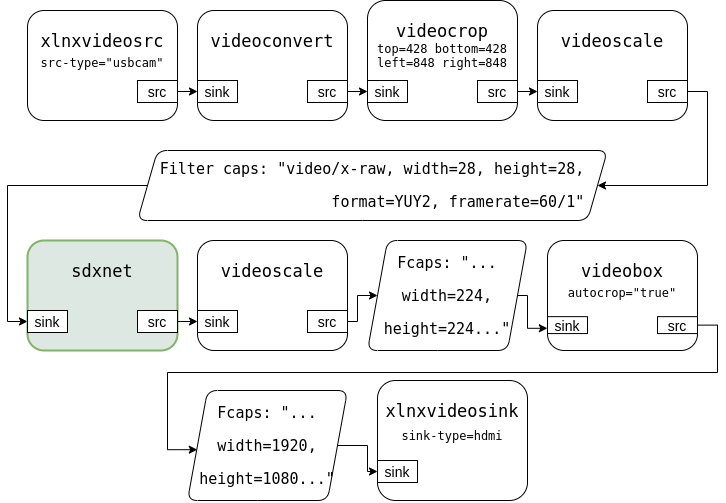
\includegraphics[scale=0.5625]{figures/pipeline.png}
  \caption{Schemat grafu. Na zielono plugin z siecią neuronową}\label{fig:pipeline}
\end{figure}
Zsyntetyzowana sieć jest częścią projektu. Potrzebne również dostarczenie
danych do sieci oraz przedstawienie wyniku.
Do tego celu skorzystano z biblioteki GStreamer, dzięki której można
tworzyć grafy z komponentów (pluginów, elementów)
przetwarzających media, zarówno audio jak i video.
Każdy z elementów grafu składa się z co najmniej jednego źródła (source),
lub ujścia (sink), może mieć również wiele wejść i wyjść. W grafie pierwszy
element nie może mieć wejść, natomiast konieczne jest aby posiadał co najmniej
jedno wyjście. Poprawnie przygotowany graf nie powinien mieć komponentów
oferujących źródło, które nie są z niczym połączone.
Pluginy mają ujednolicony interfejs, dzięki czemu można w łatwy sposób
włączyć do grafu własny element. Wtyczki charakteryzują się
pewnymi własnościami, znanymi jako „caps”. Określają one jakie 
media jest w stanie przetworzyć dana wtyczka (na przykład format pikseli,
maksymalny rozmiar obrazu). 
Łączone ze sobą elementy dokonują negocjacji
parametrów mediów, takich jak rozdzielczość obrazu, format pikseli,
ilość klatek na sekundę oraz innych.

\todo[inline]{Elementy wypisać z opisem
  alfabetycznie czy zgodnie z kolejnością elementów w pipeline?}

\subsubsection{Filter caps}
Element precyzujący parametry obrazu, które wymuszają
dostosowanie się poprzedniego elementu --- na przykład videoscale.
Zapisuje się je w postaci ciągu znaków objętych w cudzysłów.

\subsubsection{fpsdisplaysink}
Wtyczka typu sink (mająca tylko ujście), która jako parametr
pobiera inną wtyczkę tego typu, np.~xlnxvideosink. Jej użycie
pozwala na sprawdzenie liczby klatek na sekundę wyświetlanego
obrazu.

\subsubsection{videobox}
Oferuje możliwość osadzenia obrazu w tym o innym rozmiarze
rozmiarze wypełniając pozostałą przestrzeń ramką
w wybranym kolorze. Własność autocrop oznacza automatyczne obliczenie
wielkości ramek na podstawie parametrów określonych przez kolejny element tak,
aby obraz przychodzący do videobox był wycentrowany a ramki
były tej samej wielkości.

\subsubsection{videoconvert}
Element mający za zadanie dostosować wszystkie parametry obrazu tak,
aby móc połączyć ze sobą dwa niekompatybilne pod względem „caps” elementy.
Ta niekompatybilność może być spowodowana na przykład tym, że dwie
wtyczki potrzebują innego formatu pikseli i jednocześnie nie oferują
możliwości konwersji z jednego formatu na inny.

\subsubsection{videocrop}
Wtyczka służąca do wykadrowania obrazu w zdefiniowanym obszarze.
Wykorzystana została aby otrzymać obraz o tej samej długości
i szerokości wynoszącej 224 (co jest ośmiokrotnością 28, czyli
długością boku obrazów, którymi wytrenowana została sieć) wycięty
ze środka wideo o rozmiarze 1920\(\times \)1080.

\subsubsection{videoscale}
Skaluje obraz do wynegocjowanych pomiędzy sąsiadującymi elementami
parametrów, przy czym pierwsza próba negocjacji to ta sama wielkość
obrazu przy ujściu jak i w źródle, aby skalowanie nie było potrzebne.

\subsubsection{xlnxvideosrc i xlnxvideosink}
Są to pluginy dostarczone przez firmę Xilinx wraz z platformą reVISION.
Obydwa korzystają biblioteki Xilinx \lstinline{video_lib}
Pierwszy z nich ułatwia odczytywanie danych ze źródeł, dla których potrzebne
byłyby dodatkowe działania. Są to między innymi kamera USB (użyta w projekcie),
HDMI, MIPI CSI (sprzętowy interfejs do transmisji obrazów i wideo).
\todo{Przypis UG1221, s.32}
Sam element zbudowany jest w oparciu o element v4l2src, dostępny
w standardowej instalacji GStreamera.
Xlnxvideosink również jest oparty o inny element --- kmssink.
Zapewnia odpowiednią konfigurację połączenia z wyświetlaczami
podłączonymi przez HDMI oraz DisplayPort.


\subsection{Używanie sieci}
\subsubsection{Generowanie projektu}
Architekturę sieci wraz z wagami zapisano do pliku h5. Stworzono
plik konfiguracyjny hls4ml. Następnie na jego podstawie wygenerowano projekt
z przekonwertowaną siecią. Wśród wygenerowanych plików znajduje się
również kod służący do symulacji działania projektu. Przygotowane zostały
pliki z danymi testującymi sieć --- 10000 przetworzonych przykładów z bazy
MNIST tak, aby cyfry były koloru czarnego, tło białego. Zakres wartości
wynosi od 0 do 255.

\subsubsection{Funkcja}
Cała sieć jest przedstawiona jako jedna funkcja.
Parametrami tej funkcji są dwie tablice:
\lstinline[style=hls]{input[]}, do której są zapisywane są
dane do przetworzenia,
oraz \lstinline[style=hls]{output[]}, do której funkcja zapisuje
obliczone predykcje.

\begin{minipage}{\linewidth}
\lstinputlisting[
  caption={Nagłówek funkcji},
  label={lst:nn_header},
  style=hls
]{listings/nn.h}
\end{minipage}

\subsubsection{Interfejs}
Aby móc korzystać z sieci w aplikacji uruchamianej na procesorze ARM
zadeklarowano użycie interfejsu IO \mbox{AXI-4} Lite.

\subsubsection{Dostosowanie sieci}
W celu poprawienia wyników działania sieci dokonano pewnych usprawnień.
Sieć została wytrenowana oryginalnymi danymi, w których piksele tworzące
cyfry mają wartości równe 255 lub tej wartości bliskie,
a piksele białego są przedtawione jako 0.
Ponadto rzeczywiste dane z kamery mogą być zaszumione,
przedstawione obiekty zacienione, a same cyfry mogą nie być idealnie czarne.

Przy każdym wywołaniu funkcji sieci dokonywana jest transformacja
danych poprzez kod pokazany na listingu~\ref{lst:data_tresh}.
Wartość każdego z piksela jest zamieniana na wartość 255 lub 0, zależnie
od początkowej jego wartości --- dla wartości mniejszych od 140
(kolor szary lub ciemniejszy) przypisany jest kolor biały, wartość 255.
Dla pikseli jasnych (od 140 w górę) przypisywana wartość to 0, kolor czarny.

W ten sposób dokonuje się zarówno odpowiedniego przetworzenia danych
uwzględniającego sposób wytrenowania modelu, jak również uwydatnienia
cyfry oraz pozbycia się szumów obrazu i jasnych cieni.

\hspace{-1cm}
\begin{minipage}{\linewidth}
\lstinputlisting[
  caption={Transformacja danych.},
  label={lst:data_tresh},
  firstline=36,
  lastline=39,
  language=C++
  % floatplacement=H
]{listings/nn.cpp}
\begin{itemize}
  \setlength{\itemindent}{3em}
  \item \lstinline[style=hls]{input[]} --- tablica z danymi (parametr funkcji)
  \item \lstinline[style=hls]{input1[]} --- dane przetwarzane przez sieć
\end{itemize}
\end{minipage}

\subsubsection{Tworzenie biblioteki}
\begin{figure}[h]
\todo[inline]{Rysunek tymczasowy, zostanie zastąpiony własnym w lepszej jakości}
  \centering
  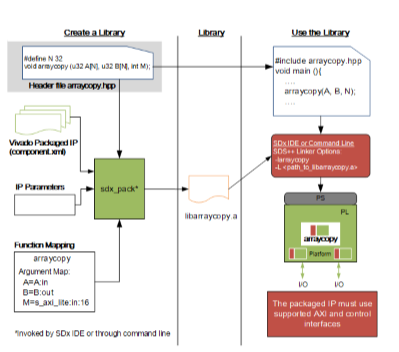
\includegraphics[scale=0.7]{figures/c-call.png}
  \caption{Schemat tworzenia biblioteki}\label{fig:ccall}
\end{figure}
Zsyntetyzowany moduł sieci został wyeksportowany w środowisku Vivado HLS
do paczki IP (Intelectual Property). Następnie poprzez narzędzie
\lstinline{sdx_pack} utworzono statyczną bibliotekę gotową do wykorzystania
w innym projekcie w środowisku SDSoC (Software-Defined System on Chip,
IDE do pisania aplikacji lub bibliotek uruchamianych na platformach
Xilinx MPSoC).

\begin{minipage}{\linewidth}
\lstinputlisting[
  caption={Narzędzie sdx\_pack},
  label={lst:sdx_pack},
]{listings/sdx_pack.sh}
\end{minipage}

Wywołując narzędzie \lstinline{sdx_pack} należy podać plik nagłówkowy funkcji,
docelową nazwę biblioteki, mapowanie parametrów funkcji na porty modułu,
ścieżkę do pliku \lstinline{component.xml} wygenerowanego podczas eksportu
do paczki IP, protokół kontroli modułu, odpowiedni zegar, a informacje
dotyczące docelowej platformy: nazwę jej rodziny, procesora oraz systemu.

\subsection{Część neuralnet}
Czytanie obrazu, podział na część luma i chroma, wywołanie funkcji sieci,
zapis z powrotem, synteza do biblioteki dzielonej „.so”

\subsection{Część gstsdxnet}
De facto plugin gstreamera, w którym są wywoływane funkcje z biblioteki
dzielonej neuralnet.so, 

\subsection{Małe podsumowanie}


\newpage
\section{Wyniki i dyskusja}

\subsection{Ewaulacja modelu}
Wyniki z samego pythona z danymi testowymi z mnista

\subsection{Symulacja}
Tutaj wyniki z symulacji z danymi testowymi z mnista

\subsection{Dane rzeczywiste}
Wyniki z kamerki. Zdjęcia danych testowych, co wpływa na wynik, czy wszystko
rozpoznaje itd,

\newpage
\section{Podsumowanie}
W projekcie zostało zrobione to i to. Wyszło to tak i tak. Problem sprawiło
tamto i owamto. Można to poprawić w ten sposób. Można część funkcjonalności
z pipeline przenieść na fpga (w końcu przetwarzanie obrazu na fpga jest szybkie)

\end{document}